\section{Analysis}
\subsection{Problem Defenition}
The goal of this project is to design the hardware specification for a custom 16-bit single cycle CPU, and develop the suite of tools required to simulate such a processor, including an Emulator (\ref{sec:Emulator}), Assembler (\ref{sec:Assembler}), and Compiler (\ref{sec:Compiler}). The project will detail the abstract design of the computer’s Instruction Set Architecture (ISA) (\ref{sec:ISA}) and its implementation in hardware, considering the internal registers, system clock, main memory, and fetch execute cycle.

The project will compose three primary parts, an emulator capable of loading machine code 'catridges' and simulating the hardware, memory, peripherals and registers detailed by the ISA in order to execute programs with correct clock timing and behaviour. An assembler to translate programs written in an assembly specification into binary machine code (the assembler will handle higher level conveniences such as relative addressing through labels). And finally a compiler - to translate a higher level programming langauge into machine code. This will require compiler optimisations with relation to the produced object code; complex data structures such as arrays, objects and strings; conditional and interative expressions; and functions and procedures. The suite required to simulate such a computer should be capeable of writing and compiling complex programs such as pong or tetris, and emulating them with hardware correct timings - dealing with peripherals such as a keyboard or speaker.

\subsection{Background to the Problem Area}
This project will explore lower level systems software and look in detail at the fundemental architecture of modern computing systems and how they are designed from the ground up.

\subsubsection{Instruction Set Architecture}
\label{sec:ISA}
The ISA acts as an interface between the hardware and software of a computing system, and contains crucial information regarding the capabilities of a processor, including: a functional defenition of storage locations (e.g. registers and memories) as well as a description of all instructions and operations supported.

An ISA can be classified according to its architectural comlpexity into a Complex Instruction Set Computer (CISC), or a Reduced Instruction Set Computer (RISC). A CISC processor implements a wide variety of specialized instructions in hardware (e.g. floating point arithmetic or transferring multiple registers to or from the stack), minimising the number of instructions per program at the cost of a more complex design, higher power consumption and slower execution as each instruction requires more processor cycles to complete. \textcite{gfg-risc-vs-cisc} Thus optimisations in performance occur on the hardware level. This is historically the most common branch of processor and often results in processors with large instruction sets, for example the Intel x86's 1503 defined instructions \textcite{ryg-blog}. A RISC processor however aims to simplify hardware using an instruction set consisting of a few basic instructions to load, evaluate and store data - instead placing optimisations on the software side unlike a CISC processor. This has the side effect of increased memory usage required to store additional instructions needed to perform complex tasks.

\subsubsection{Emulator}
\label{sec:Emulator}
An emulator is a software program that allows one computer to imitate another - and by simulating the hardware of the other – execute machine code programs written for a processor other than itself. Emulators tend to consist of three modules, a CPU emulator, memory subsystem module, and I/O device emulators \textcite{retroreversing}. The simplest form of CPU emulator is an interpreter - wherein the emulator steps sequentially through each machine code instruction, and carries out the fetch-decode-execute cycle for each, modifying the internal state of the simulated processor in the same manner as the instruction would affect the physical hardware - this can be achieved by representing internal flags and registers as variables. The Memory Subsystem can be implemented as a one dimensional array of bytes - with features such as memory mapped I/O implemented by associating regions of memory to peripherals and subsystems, e.g. Video Random Access Memory (VRAM), the stack, and the heap. 

\subsubsection{Assembler}
\label{sec:Assembler}
An assembler is a program that translates assembly language (a low level programming language that uses mneumonics to directly represent machine code instructions) into object code that can be executed by the processor. There are 2 types of assembler design, single-pass and multi-pass \textcite{TOPPR-assembler}. A single-pass assembler scans the source code only once to translate it into machine code, and outputs the result directly. This is a simpler type of assembler, and is more efficient with regard to translation speed. However, it requires all symbols used within the program (variables, labels, etc...) to be declared before they are used - else the program will crash. 

A multi-pass assembler however scans the source code multiple times, on the first pass defining a symbol table and opcode table \textcite{TOPPR-assembler}, processes pseudo instructions (compound macro instructions that are substituted during assembly with a list of fundemental instructions), and maintaining a location counter to store the memory address of each instruction as it would be compiled.

There are also certain higher level abstractions a high-level assembler can translate such as \texttt{IF/THEN/ELSE/WHILE} statements and certain higher level data types – however this results in a complex assembler and lengthy compilation times - as well as a blurred line between the role of high level and low level languages. 

\subsubsection{Compiler}
\label{sec:Compiler}
A compiler is a program that translates high level program source code into a set of machine language instructions. Some compilers translate source code into an intermediate assembly language before using an assembler to produce the machine code instructions, whereas others compile into machine code directly. The typical pipeline to any compiler is depicted in fig. \ref{fig:compiler-pipeline} \textcite{Ball-WritingACompilerInGo}.

\bigskip

\begin{figure}%
    \centering
    \subfloat[\centering Compiler Pipeline]{{
        \shadowbox{
            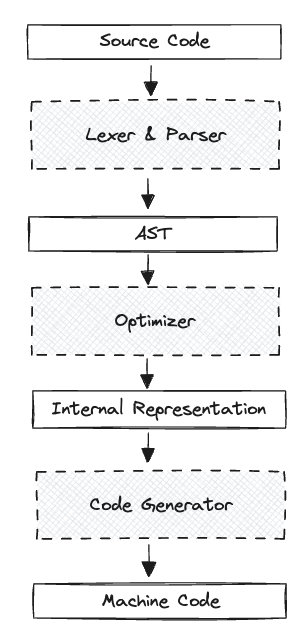
\includegraphics[height=6cm]{Screenshot 2024-04-21 at 14.52.32.png}
        }
        \label{fig:compiler-pipeline}%
        }}%
    \qquad
    \subfloat[\centering Abstract Syntax Tree]{{
        \shadowbox{
            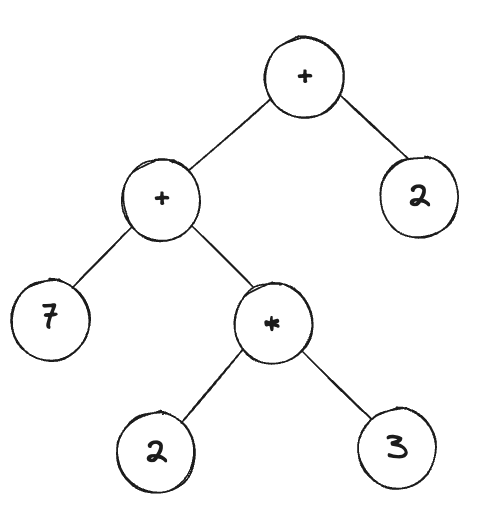
\includegraphics[height=6cm]{Screenshot 2024-04-21 at 15.01.11.png}
        }
        \label{fig:ast}%
    }}%
\end{figure}

\bigskip


The ASCII source code is tokenised by the lexer, and transformed into an Abstract Syntax Tree (AST) by the Parser. The AST is a means of breaking down the program, its statements, and order of operations into a tree representation that is easier to be processed and traversed by an algorithm. The AST representing expression ($\frac{7+2\times3}{2}$) depicted in fig. \ref{fig:ast}. The optimizer may convert the AST into an Internal Representation (IR) (be that binary, textual, or another syntax tree) that may lend itself better to optimisations and translation into the target language than the AST. From this new IR, optimisations may include eliminating dead code, precalculating simple arithmetic, and numerous other optimisations \textcite{Ball-WritingACompilerInGo}. Finally, the code generator generates the optimised code in the target language (compilation) and is stored as a file on the user's computer.

\bigskip

\bigskip

\subsubsubsection{Lexer}
The lexer steps through the ASCII source code character by character and builds up tokens representing the basic elements of programs such as a String, Integer, Identifier, Operation. For example the program: \texttt{print("Result: ", (answer+1)/2)} would be tokenised as:

\begin{lstlisting}
IDENTIFIER("print"), LPAREN, String("Result: "), COMMA, LPAREN, IDENTIFIER("answer"), ADD, INTEGER(1), RPAREN, DIV, INTEGER(2), RPAREN
\end{lstlisting}

This process of tokenising the program string into a series of objects makes it easier to parse into an AST and for the parser to step through by element rather than character.

\subsubsubsection{Parser}
The process of converting the list of tokens representing the program generated by the Lexer into a tree representation (AST) that reflects the order of operations and sequence of statements is called Parsing. And is carried out by a Parser. A common algorithm used for parsing programs is a Pratt parser due to its concise nature and extensibility. 

\subsubsubsection{Optimization \& Code Generation}
Code generation is the process of converting the AST generated from the Parser into an intermediate language which itself can be compiled down to an executable or interpreted by a virtual machine. For my NEA, the compiler will first compile down into assembly language - which will then be assembled into the executable machine code - simplifying compilation through the available higher level functionality such as labels and offsets. Each higher level statement typically templates onto a standard sequence of machine code instructions, for example a program to add 2 numbers:
\begin{lstlisting}
let a = 9;
let b = 5;
let c = a + b;
\end{lstlisting}

May compile down into the following assembly language:
\begin{lstlisting}
ldi R0, 9
ldi R1, 5
add R2, R0, R1
\end{lstlisting}
Compilations such as these involve the mapping of a potentially infinite number of variables to a discrete number of regiseters and this can be performed using such algorithms as the Linear Scan or Chatins' algorithm \textcite{GFG-linearscan} that take into account variable lifetimes and interactions. Offsets required for branch instructions that may be used in iterative or selective statements can be calculated by counting the number of instructions compiled up to the point of a particular statement (e.g. the number of machine code instructions up the the condition of a while loop) and this can be used as either an absolute or relative offset depending on the capabilities of the assembler.

\subsection{Existing Systems}
\subsubsection{University of Washington MIPS Computer}
The following system is a 16 bit MISC (Minimal Instruction Set Computer) processor designed by the University of Washington for a series of lectures as part of their computer science course \textcite{MIPS-uw}, and I will discuss its ISA and machine code encoding - to aid my design of an appropriate and efficient computer architecture. A MISC processsor is a subclass of the RISC processor and involves minimising the number of instructions implemented in hardware, resulting in far simpler hardware designs - where a RISC processor may have 30-70 instructions, a MISC processor may have merely 10-20 consisting of arithmetic, branching, loading and storing instructions. \textcite{MISC-dakeng}. 

A MIPS (Microprocessor without Interlocked Pipelined Stages) processor such as this does not overlap the execution of several instructions (pipelining), thus neglecting the potential performance gains in favor of a simpler architecture. This processor is a single-cycle implementation meaning all instructions take exactly one cycle to complete, this is achieved using a Harvard architecture in place of Von Neuman wherein instructions are stored in a seperate Read Only Memory (ROM) to data, thus both can be fetched within the same processor cycle. 

The processor supports the following instructions:
\begin{enumerate}
    \item Arithmetic \texttt{add, sub, and, or, slt (set if less than)}
    \item Data Transfer \texttt{lw (load word), sw (store word)}
    \item Control \texttt{beq (branch if equal to)}
\end{enumerate} 
Register-to-Register arithmetic instructions use the R-type encoding for their machine code representation, where \texttt{op} is the opcode of the instruction with \texttt{func} representing the particular arithmetic operation. \texttt{rs, rt}, and \texttt{rd} are the source and destination registers. This computer operates on an ALU with a 3 bit control signal supporting 5 operations that directly correspond to the \texttt{func} portion of an R type instructions binary encoding. 

\bigskip

\shadowbox{
    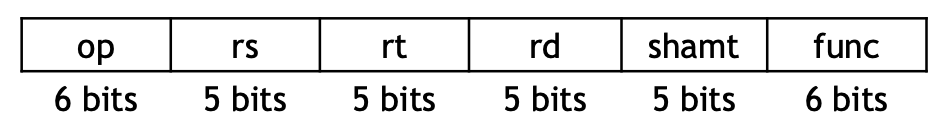
\includegraphics[width=11cm]{Screenshot 2024-04-14 at 22.19.47.png}
}

\bigskip

The I type encoding is the second means for which instructions can be represented, and includes the data transfer and control instructions \texttt{lw, sw}, and \texttt{beq} specified above. \texttt{address} is a signed 16 bit constant. \texttt{rt} is the destination for \texttt{lw} and source for \texttt{beq} and \texttt{sw}. \texttt{rs} is the base register for the \texttt{lw} and \texttt{sw} instructions (added to the sign extended constant \texttt{address} to get a data memory address) \textcite{MIPS-uw}. In this processor design, for a \texttt{beq} instruction, the \texttt{address} field specifies not a memory address, rather a signed offset from which to jump from the current PC position when executing the branch instruction.

\bigskip

\shadowbox{
    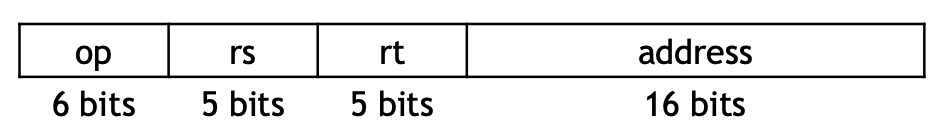
\includegraphics[width=11cm]{Screenshot 2024-04-14 at 22.33.16.png}
}

\bigskip

Below is the full datapath specification for the computer, with the Instruction Memory (ROM) on the left, connected to the PC in order to address instructions. Those instructions are in turn passed through the control unit and decoded, with the opcode specifying whether an I or R type instruction is being processed and accordingly what hardware should be used to interpret and execute the instruction. This dictates the calculation (if any) that is to be performed in the ALU - the output of which is stored in a seperate data memory.

Since instructions are stored in a seperate ROM, the address of the first instruction will always begin at 0 - this simplifies the calculation of offsets and labels in the assembler – since the assumption that the first instruction begins at address 0 will always hold true. However, branch instructions are handled unusually in this computer - instead of specifying the jump address, the signed offset from the current instruction is specified instead. This has the effect of making compilation easier as branch addresses do not need to be calculated by the assembler, however renders specific jumps to memory addresses (such as the location of an interrupt service routine or bootloader) difficult.

\bigskip

\shadowbox{
    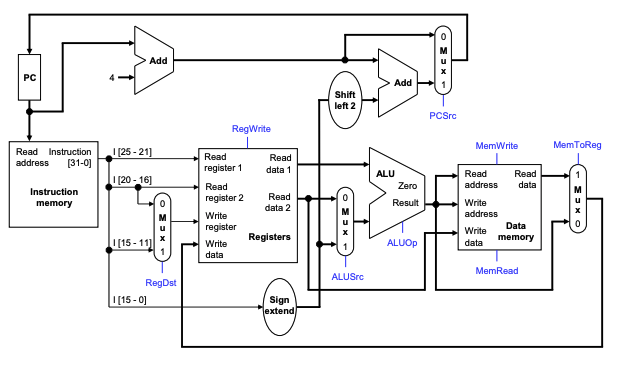
\includegraphics[width=11cm]{Screenshot 2024-04-14 at 19.42.11.png}
}

The architecture described above has some notable advantages, firstly, its Harvard architecture allows the processor to operate each instruction in a single cycle – both improving performance and simplifying the design of the emulator as microinstruction cycles do not need to be simulated  to accurately simulate the hardware. Secondly, by dividing the computer architecture into 2 distinct I and R type instructions, you can reduce redundant information – and thus the bits required to store machine code instructions and programs.

However, this simple architecture results in many inconveniences when writing assembly code - due to the limited instruction set, simple tasks take comparatively more instructions meaning programs are longer and more tedious to write - as well utilising more memory due to the limited number of specialized instructions who's functionality must be implemented using handwritten subroutines such as binary shifts, stack operations, or interrupt handling. 

\bigskip

The takeaways of this system for my project include:
\begin{enumerate}
    \item The encoding of instructions into meaningful machine code that directly relates to the hardware of the computer - for instance R type opcodes representing the control bits of the ALU, this makes decoding instructions more efficient - especially when implmented in hardware.
    \item Secondly, the behaviour of hardware (registers, memories, flags) and the relationships between components during a single-cycle Harvard fetch-execute cycle that will have to be simulated when designing an emulator.
    \item I will also expand the instruction set further than the MISC specification used in this processor to include other common instructions, and keep the memory-register seperation wherin operations are performed on register values, with 2 instructions \texttt{lw, sw} used for reading and writing to memory.
    \item I will also change the branch instruction to operate on absolute addresses rather than signed offsets.
\end{enumerate}

\subsubsection{The Hack Computer}
The Hack computer is a theoretical 16 bit computer designed by Noam Nisan and Shimon Schocken and described in their book The Elements of Modern Computing Systems \textcite{EOCS}, I will analyse its method of encoding assembly instructions into machine code - as well as the syntax of its assembly language to inform my assembler design and machine code specification. The Hack computer contains 2 16-bit registers labelled A and D, the D (data) register is a general purpose register that always acts as 1 of the 2 inputs to the ALU. Wheras the A (address) register has 2 functions: a second signed integer value for ALU operations, and a target address in instruction memory or data memory addressing. The pseudo-M (memory) register is not implemented in hardware - rather refers to the word in RAM addressed by the A register and therefore can be used to directly interract and perform calculations with memory.
\begin{lstlisting}
A type: 0aaaaaaaaaaaaaaa
C type: 111accccccdddjjj
\end{lstlisting} 
Hack takes a unique aproach to ISA design through its address instructions (A-type) and computational instructions (C-type). The first bit of any machine code instruction determines its type. For an A instruction - the latter 15 bits store the data (or address) as which to set the A register (\texttt{a}). 

For a C-type instruction the the first 2 bits of the 15 bit operand remain unused and set to 1 by standard, this is followed by the 1 bit addressing mode (\texttt{a}) which determines whether A or M is used as the ALU's second input. Then, the computation specification (\texttt{c}) composes the next 5 bits, and dictate which operation the ALU will perform, directly mapping to the ALU's control bits \textcite{EOCS}. Following, the 3 bit destination specifier (\texttt{d}) in turn relate to the 3 'registers' A, D, and M. Should their corresponding bit be set the ALU output will be stored in the A, D or M registers (potentially multiple). The final 3 bits describe the jump condition - each Hack C type instruction is terminated by a branch (which can be left blank). They relate to the Less Than, Equal to, or Greater Than conditions respectively, and a combination can be used to form all conditionals.

\bigskip

\shadowbox{
    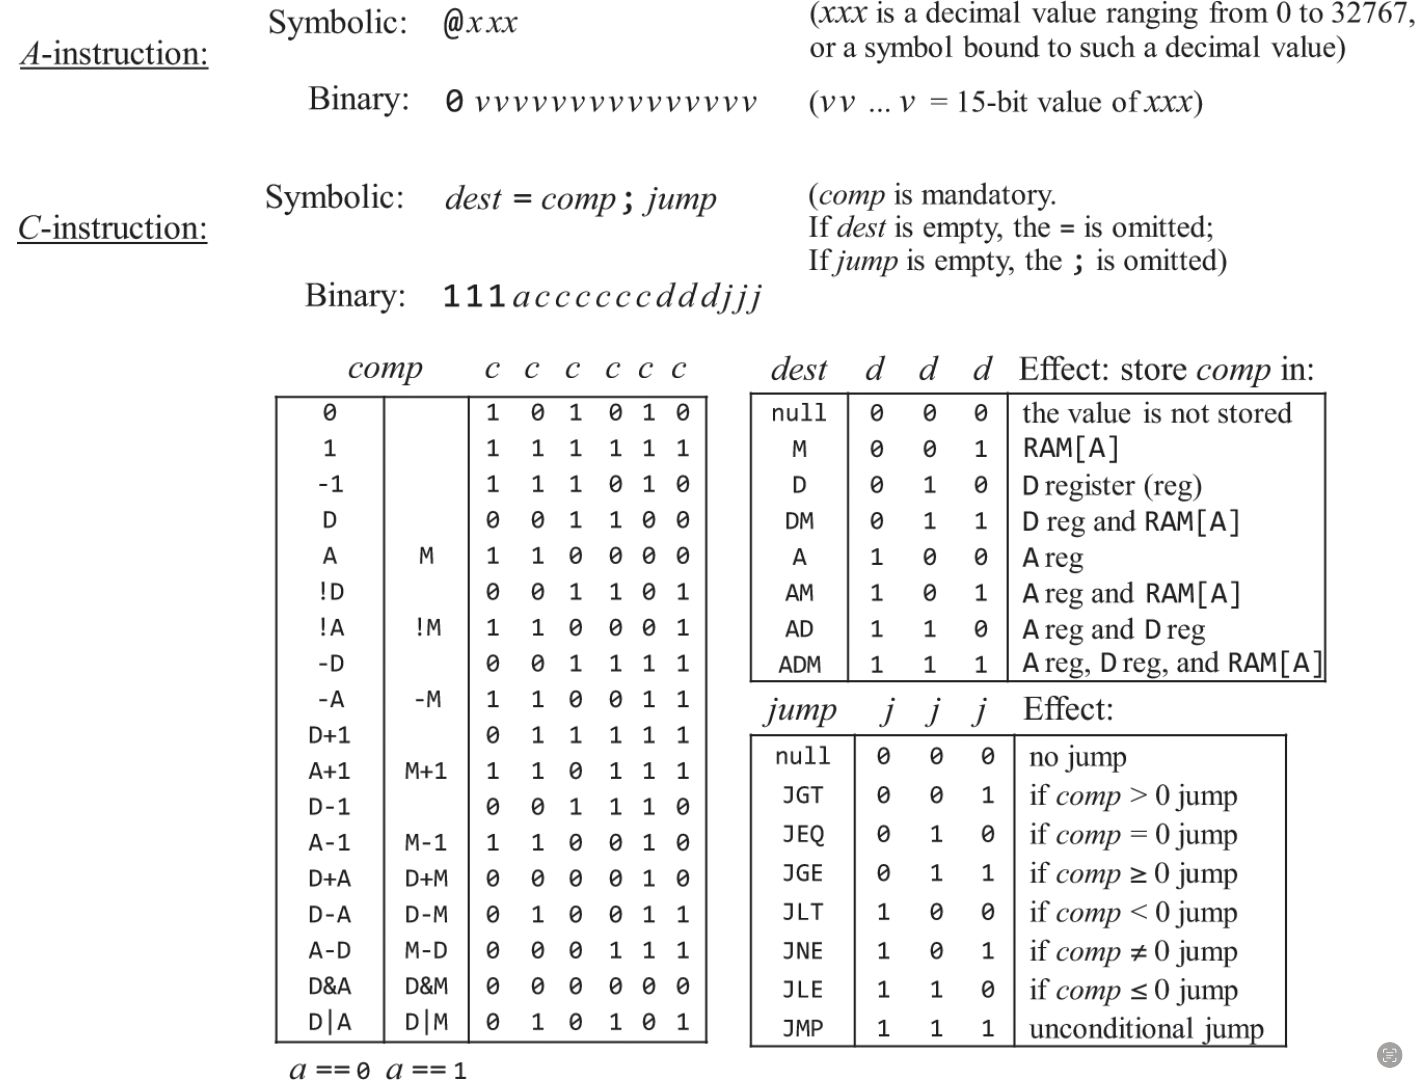
\includegraphics[width=11cm]{Screenshot 2024-04-21 at 17.17.34.png}
}

\bigskip

This approach to ISA design being so fundementally related to the internal operations of the CPU comes with some advantages and disadvantages. Firstly, it is a very efficient design - allowing all essential operations to be carried out with a simple computer architecture. This simplicity makes it an ideal compilation target. However, Hack assembly can be unintuitive to write and understand - especially in relation to its Harvard architecture and thus simultaneous addressing of both instructions and data from ROM or RAM respsectively. An example Hack assembly program might look as follows:
\begin{lstlisting}
// i = 1
@i
M = 1

(LOOP)
    // if (i > 10) goto STOP
    @i 
    D = M

    @10
    D = D - A

    @STOP
    D; JGT

    // i += 1
    @i
    M = M + 1

    // goto LOOP
    @LOOP
    0;JMP
(STOP)
@END
0; JMP
\end{lstlisting}

Hack's approach to assembly is also worth considering, It uses parenthesis to specify labels (points in the code from which instructions can branch to without specifying a numeric offset). The '@' character is used to specify an A type instruction - however using an identifier as the operand is a high level assembler abstraction that at compile time replaces all occurrences of the identifier with a calculated memory address representing that variable. All C-type instructions are in the form \texttt{<destination(s)> = (<destination> <operation> <destination>)? (; <branch>)?} where the branch expression components of the instruction are optional. 

To compile this down into machine code (once labels have been replaced with offsets) - the A instruction is simply the 15 bit operand. The C instruction however is more involved. A lookup table is used to map the operations (\texttt{+, -, /, *, !, \&}) into 5 bit opcodes (with the first bit of the 6 bit computation specified determined by whether the A or M registers are included in the operands). Then the bit corresponding to each destination specified will be set, and finally the conditional branch bits will be set depending on the mneumonic used, e.g. \texttt{JGE} would be replaced by \texttt{011}. Together, the instruction \texttt{D = D - A; JNE} would be represented by the binary \texttt{111 010011 010 101}. 

From this case study, there are a number of takeaways:
\begin{enumerate}
    \item Breakdown instructions into types capable of representing a family of assembly insstructions - reducing the number of machine code instructions required to be implemented by the virtual machine.
    \item Use a pseudo-register to represent the addressing behaviour of a Harvard architecture computer, simplifying operations involving memory access \& compilation behaviour.
    \item Represent branch conditionals through 3 bits reflecting \texttt{<, =, >} comparisons  
    \item Use one bit to represent each destination register allowing for a combination of destinations for a paricular instruction meaning seperate instructions need not be created for storing data in memory or registers.
\end{enumerate}

\subsubsection{Monkey}
Monkey is the programming language described in Thorsten Ball's book Writing a Compiler in Go \textcite{Ball-WritingACompilerInGo}, I will be analysing the syntax of the language to inform my high-level language design. Monkey has a C-like syntax, variables, integers and booleans, arithmetic expressions, first class functions (functions that can be passed to other functions as parameters), strings, and arrays. Its syntax looks as follows:
\begin{lstlisting}
let fibonacci = fn(x) {
    if (x == 0) {
        0;
    } else {
        if (x == 1) {
            1;
        } else {
            fibonacci(x - 1) + fibonacci(x - 2);
        };
    };
}

let main = fn() {
    let numbers = [1, 2, 10, 50, 9*18];
    let index = 0;

    while (index < length(numbers)) {
        print(fibonacci(numbers[index]));
        index = index + 1;
    }
}
\end{lstlisting}

This approach to language syntax is convenient to program, in particular, by representing functions as variables it allows you to pass functions as parameters (first class functions) without additional logic, however functionality as such is difficult to implement in machine code - passing the address of the first instruction rather of the function than the function itself is a more practical solution for a compiled language. References and pointers are not present in Monkey, these permit complex functionality such as arrays and strings, whilst maintaining a simple compiler - however can lead to code that is difficult to understand and takes familiarity in the hardware to write. Monkey simply interprets these using Go's built in data structures thus doesn't have to worry about compiling them into binary - meaning specifying a data type is less important.

Monkey is a dynamically typed languge - which means variable types are not checked and can result in runtime errors when attempting to add an integer to a string, or assign an integer to a float type variable. Using the \texttt{let} keyword to define a variable as above(unlike python) is vital for a compiled language - since additional functionality is required to allocate a memory address (or regiser) for that particular variable depending on its lifetime.

The takeaways from this system include:
\begin{enumerate}
    \item Using established programming language norms for defining variables, iterative statements and functions will make the programming language easier to learn due to transferable experience.
    \item Designing a statically typed language would reduce program crashes and lead to a more robust compiler and programs.
    \item Including references and pointers allow for the implementation of features such as arrays and strings whilst maintaining a concise and simple compiler.
    \item I should consider defining variables with the 'let' keyword to tell the compiler it needs to insert additional logic calculating an appropriate memory address in which to store the variable, and store that address in a lookup table against its identifier.
\end{enumerate}

\subsubsection{Jack}
Jack is the high level langauge defined in book The Elements of Modern Computing Systems \textcite{EOCS} with a syntax similar to Java. I will analyse its syntax and how it is compiled into machine code to inform my design of a compiled language. Jack is an Object-Oriented statically typed language similar to Java that is compiled down into the Hack machine code specification. An example Jack program may look as follows \textcite{EOCS}:
\begin{lstlisting}
class List {
    // declare the class attributes
    field int data;
    field List next;

    // define a constructor to initialise a List with attributes data and next
    constructor List new (int dataParam, List nextParam) {
        let data = dataParam;
        let next = nextParam;
        return this;
    }

    method int getData() { return data; }
    method List getNext() { return next; }

    method void print() {
        // declare a pointer to the first element of the list
        var List current;
        let current = this;

        // iterate through all the elements in the linked list
        while (~(current = null)) {
            do Output.printInt(current.getData());
            do Output.printChar(32) // space
            let current = current.getNext();
        }

        return;
    }
}
\end{lstlisting}


Above is the example program to define a linked list in Jack as provided in the book, and shows the similarities and differences to other popular languages. Jack has program structure very similar to that of Java, or C\# - relying on a series of classes containing program logic which can be invoked using the \texttt{do} keword. Jack splits the functionality of certain keywords in typical programming languages into more specialized roles: for instance the \texttt{field} keyword used to define object attributes, the \texttt{let} keyword being used every time when assigning to variables, the \texttt{method} and \texttt{constructor} keywords typically under the umbrella of \texttt{function}, and the \texttt{do} keyword used to invoke methods. This can introduce a steeper learning curve when learning Jack and adds complexity.

However the reason for differentiating field variables and regular variables is due to their lifetimes. A copy of field variables needs to be maintained for each instance of a paritcular class - wheras other local variables can be freed from memory once their particular subroutine terminates and they are no longer used.

To compile selection statements in the Jack Compiler, the compiler generates a series of arbitrary labels e.g. (L1, L2) and places these after key points in the selective process in order to avoid offset calculating - a functionality that can be handled by the assembler. To compile the following:
\begin{lstlisting}
if (b > 10) {
    c = b;
} elif (b % 2 == 0) {
    b = b + 1; 
} else {
    b = b - 1;
}
\end{lstlisting}

The compiler will insert labels before the first instruction of each branch, and insert any code for the unconditional 'else' block after the jump instructions for any conditions (elif, and then branches). This approach avoids calculating any offsets and thus only a single pass is required to compile this program.

\begin{lstlisting}
// if b > 10 goto .then
ldi a, 10
sub a, b, a 
bgt .then

// elif b % 2 == 0 goto .elif
ldi a, 2
mod b, 2
beq .elif

// b = b - 1
lda a, 1
sub b, a
goto end

.then
    // c = b
    mov c, b
    goto end
.elif
    // b = b + 1
    ldi a, 1
    add b, a
.end
\end{lstlisting}

The advantages of the Jack programming language include its specific keywords that offer insight into the manner in which its features are implemented - removing some of the abstraction typical higher level langauges offer. Another advantage is its type system, resulting in robust programs and reducing the edge cases a compiler would have to deal with. If an incorrect type was passed to a function or operation, an error would be thrown at compile time and no such error could occur in the compiled machine code.

However, the disadvantages of the Jack language include its Object Oriented approach making compilation difficult. Attribute variables on different instances of classes will have different  lifetimes and therefore freeeing the finite number of registers the computer offers to make space for newly declared variables becomes much harder a task. Secondly, Jack uses many unecessary keywords, for instance the \texttt{do} keyword functioning as an abstraction for calling a method and ignoring its return value, and the \texttt{let} keyword being required every time you assign a variable rather than for its declaration alone. This means declarations in Jack are required to be sepereate statements, increasing the volume of code required to perform the same task.

The takeaways from this language include:
\begin{enumerate}
    \item Use a procedural aproach to program structure rather than an object oriented one.
    \item Limit the number of keywords used in the final source code to only those that offer useful insight into the purpose of statements in the program.
    \item Use a simplified statically typed type system closer to that of Java or Go rather than Rust or C.
    \item Compile selection and iterative statements using generated labels rather than calculated offsets.
\end{enumerate}

\subsubsection{Virtual Machine Example}

\subsection{Client Proposal}
\subsubsection{Client Interview}
\subsection{Objectives}